% Options for packages loaded elsewhere
\PassOptionsToPackage{unicode}{hyperref}
\PassOptionsToPackage{hyphens}{url}
%
\documentclass[
  english,
  man,floatsintext]{apa6}
\usepackage{amsmath,amssymb}
\usepackage{lmodern}
\usepackage{ifxetex,ifluatex}
\ifnum 0\ifxetex 1\fi\ifluatex 1\fi=0 % if pdftex
  \usepackage[T1]{fontenc}
  \usepackage[utf8]{inputenc}
  \usepackage{textcomp} % provide euro and other symbols
\else % if luatex or xetex
  \usepackage{unicode-math}
  \defaultfontfeatures{Scale=MatchLowercase}
  \defaultfontfeatures[\rmfamily]{Ligatures=TeX,Scale=1}
\fi
% Use upquote if available, for straight quotes in verbatim environments
\IfFileExists{upquote.sty}{\usepackage{upquote}}{}
\IfFileExists{microtype.sty}{% use microtype if available
  \usepackage[]{microtype}
  \UseMicrotypeSet[protrusion]{basicmath} % disable protrusion for tt fonts
}{}
\makeatletter
\@ifundefined{KOMAClassName}{% if non-KOMA class
  \IfFileExists{parskip.sty}{%
    \usepackage{parskip}
  }{% else
    \setlength{\parindent}{0pt}
    \setlength{\parskip}{6pt plus 2pt minus 1pt}}
}{% if KOMA class
  \KOMAoptions{parskip=half}}
\makeatother
\usepackage{xcolor}
\IfFileExists{xurl.sty}{\usepackage{xurl}}{} % add URL line breaks if available
\IfFileExists{bookmark.sty}{\usepackage{bookmark}}{\usepackage{hyperref}}
\hypersetup{
  pdftitle={Supplimentary analyses Exploring reliability heterogeneity with multiverse analyses: Data processing decisions unpredictably influence measurement reliability},
  pdfauthor={Sam Parsons1,2},
  pdflang={en-EN},
  pdfkeywords={reliability, multiverse, analytic flexibility, data processing},
  hidelinks,
  pdfcreator={LaTeX via pandoc}}
\urlstyle{same} % disable monospaced font for URLs
\usepackage{graphicx}
\makeatletter
\def\maxwidth{\ifdim\Gin@nat@width>\linewidth\linewidth\else\Gin@nat@width\fi}
\def\maxheight{\ifdim\Gin@nat@height>\textheight\textheight\else\Gin@nat@height\fi}
\makeatother
% Scale images if necessary, so that they will not overflow the page
% margins by default, and it is still possible to overwrite the defaults
% using explicit options in \includegraphics[width, height, ...]{}
\setkeys{Gin}{width=\maxwidth,height=\maxheight,keepaspectratio}
% Set default figure placement to htbp
\makeatletter
\def\fps@figure{htbp}
\makeatother
\setlength{\emergencystretch}{3em} % prevent overfull lines
\providecommand{\tightlist}{%
  \setlength{\itemsep}{0pt}\setlength{\parskip}{0pt}}
\setcounter{secnumdepth}{-\maxdimen} % remove section numbering
% Make \paragraph and \subparagraph free-standing
\ifx\paragraph\undefined\else
  \let\oldparagraph\paragraph
  \renewcommand{\paragraph}[1]{\oldparagraph{#1}\mbox{}}
\fi
\ifx\subparagraph\undefined\else
  \let\oldsubparagraph\subparagraph
  \renewcommand{\subparagraph}[1]{\oldsubparagraph{#1}\mbox{}}
\fi
% Manuscript styling
\usepackage{upgreek}
\captionsetup{font=singlespacing,justification=justified}

% Table formatting
\usepackage{longtable}
\usepackage{lscape}
% \usepackage[counterclockwise]{rotating}   % Landscape page setup for large tables
\usepackage{multirow}		% Table styling
\usepackage{tabularx}		% Control Column width
\usepackage[flushleft]{threeparttable}	% Allows for three part tables with a specified notes section
\usepackage{threeparttablex}            % Lets threeparttable work with longtable

% Create new environments so endfloat can handle them
% \newenvironment{ltable}
%   {\begin{landscape}\centering\begin{threeparttable}}
%   {\end{threeparttable}\end{landscape}}
\newenvironment{lltable}{\begin{landscape}\centering\begin{ThreePartTable}}{\end{ThreePartTable}\end{landscape}}

% Enables adjusting longtable caption width to table width
% Solution found at http://golatex.de/longtable-mit-caption-so-breit-wie-die-tabelle-t15767.html
\makeatletter
\newcommand\LastLTentrywidth{1em}
\newlength\longtablewidth
\setlength{\longtablewidth}{1in}
\newcommand{\getlongtablewidth}{\begingroup \ifcsname LT@\roman{LT@tables}\endcsname \global\longtablewidth=0pt \renewcommand{\LT@entry}[2]{\global\advance\longtablewidth by ##2\relax\gdef\LastLTentrywidth{##2}}\@nameuse{LT@\roman{LT@tables}} \fi \endgroup}

% \setlength{\parindent}{0.5in}
% \setlength{\parskip}{0pt plus 0pt minus 0pt}

% \usepackage{etoolbox}
\makeatletter
\patchcmd{\HyOrg@maketitle}
  {\section{\normalfont\normalsize\abstractname}}
  {\section*{\normalfont\normalsize\abstractname}}
  {}{\typeout{Failed to patch abstract.}}
\patchcmd{\HyOrg@maketitle}
  {\section{\protect\normalfont{\@title}}}
  {\section*{\protect\normalfont{\@title}}}
  {}{\typeout{Failed to patch title.}}
\makeatother
\shorttitle{Reliability multiverse}
\keywords{reliability, multiverse, analytic flexibility, data processing}
\usepackage{csquotes}
\usepackage{float}
\usepackage{caption}
\usepackage{newunicodechar}
\floatplacement{figure}{H}
\raggedbottom
\ifxetex
  % Load polyglossia as late as possible: uses bidi with RTL langages (e.g. Hebrew, Arabic)
  \usepackage{polyglossia}
  \setmainlanguage[]{english}
\else
  \usepackage[main=english]{babel}
% get rid of language-specific shorthands (see #6817):
\let\LanguageShortHands\languageshorthands
\def\languageshorthands#1{}
\fi
\ifluatex
  \usepackage{selnolig}  % disable illegal ligatures
\fi
\newlength{\cslhangindent}
\setlength{\cslhangindent}{1.5em}
\newlength{\csllabelwidth}
\setlength{\csllabelwidth}{3em}
\newenvironment{CSLReferences}[2] % #1 hanging-ident, #2 entry spacing
 {% don't indent paragraphs
  \setlength{\parindent}{0pt}
  % turn on hanging indent if param 1 is 1
  \ifodd #1 \everypar{\setlength{\hangindent}{\cslhangindent}}\ignorespaces\fi
  % set entry spacing
  \ifnum #2 > 0
  \setlength{\parskip}{#2\baselineskip}
  \fi
 }%
 {}
\usepackage{calc}
\newcommand{\CSLBlock}[1]{#1\hfill\break}
\newcommand{\CSLLeftMargin}[1]{\parbox[t]{\csllabelwidth}{#1}}
\newcommand{\CSLRightInline}[1]{\parbox[t]{\linewidth - \csllabelwidth}{#1}\break}
\newcommand{\CSLIndent}[1]{\hspace{\cslhangindent}#1}

\title{Supplimentary analyses Exploring reliability heterogeneity with multiverse analyses: Data processing decisions unpredictably influence measurement reliability}
\author{Sam Parsons\textsuperscript{1,2}}
\date{}


\authornote{

Submitted to Meta-Psychology. Click here to follow the fully transparent editorial process of this submission. Participate in open peer review by commenting through hypothes.is directly on this preprint.

This work was supported by an ESRC grant {[}ES/R004285/1{]}

I would like to thank Ana Todorovic for her insightful feedback on an earlier version of this manuscript.

Correspondence concerning this article should be addressed to Sam Parsons, Cognitive Neuroscience Department, Donders Institute for Brain, Cognition and Behavior, Radboud University Medical Center, Nijmegen, the Netherlands. E-mail: \href{mailto:sam.parsons@radboudumc.nl}{\nolinkurl{sam.parsons@radboudumc.nl}}

}

\affiliation{\vspace{0.5cm}\textsuperscript{1} University of Oxford\\\textsuperscript{2} Radboud University Medical Center}

\abstract{
Contains supplimental analyses for the main paper. Specifically, the same analyses including only half of the trials.
}



\begin{document}
\maketitle

\begin{figure}
\centering
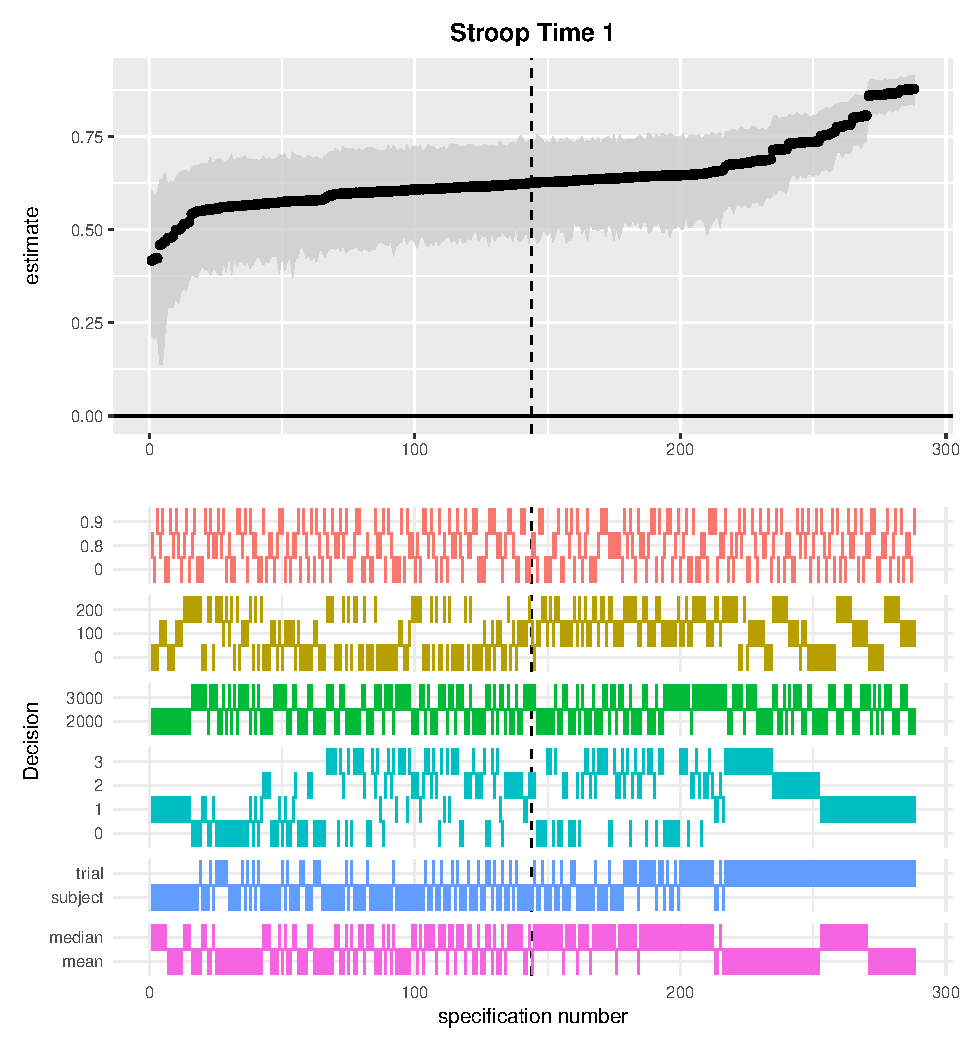
\includegraphics{half_trials_files/figure-latex/unnamed-chunk-1-1.pdf}
\caption{\label{fig:unnamed-chunk-1}Internal consistency reliability multiverse for Stroop RT cost at time 1}
\end{figure}

\begin{figure}
\centering
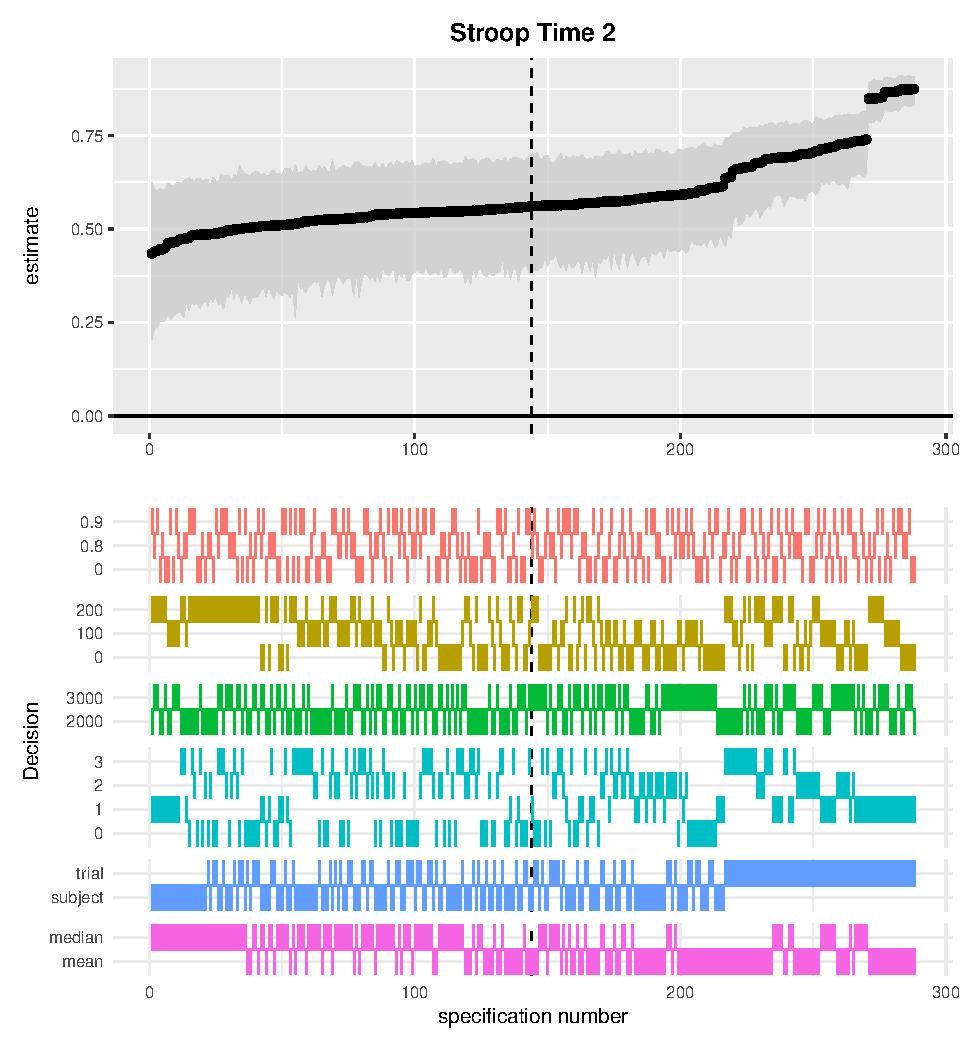
\includegraphics{half_trials_files/figure-latex/unnamed-chunk-2-1.pdf}
\caption{\label{fig:unnamed-chunk-2}Internal consistency reliability multiverse for Stroop RT cost at time 2}
\end{figure}

\begin{figure}
\centering
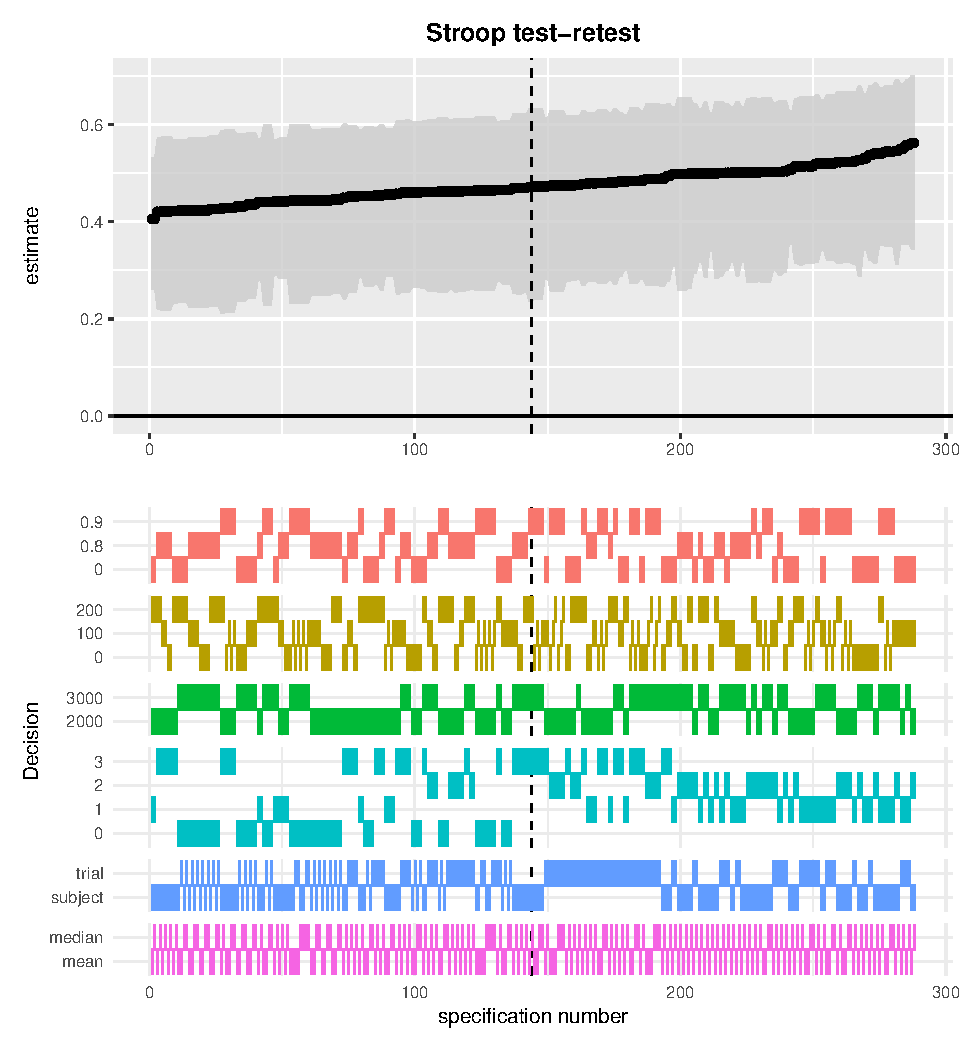
\includegraphics{half_trials_files/figure-latex/unnamed-chunk-3-1.pdf}
\caption{\label{fig:unnamed-chunk-3}Test-retest reliability multiverse for Stroop RT cost}
\end{figure}

\begin{figure}
\centering
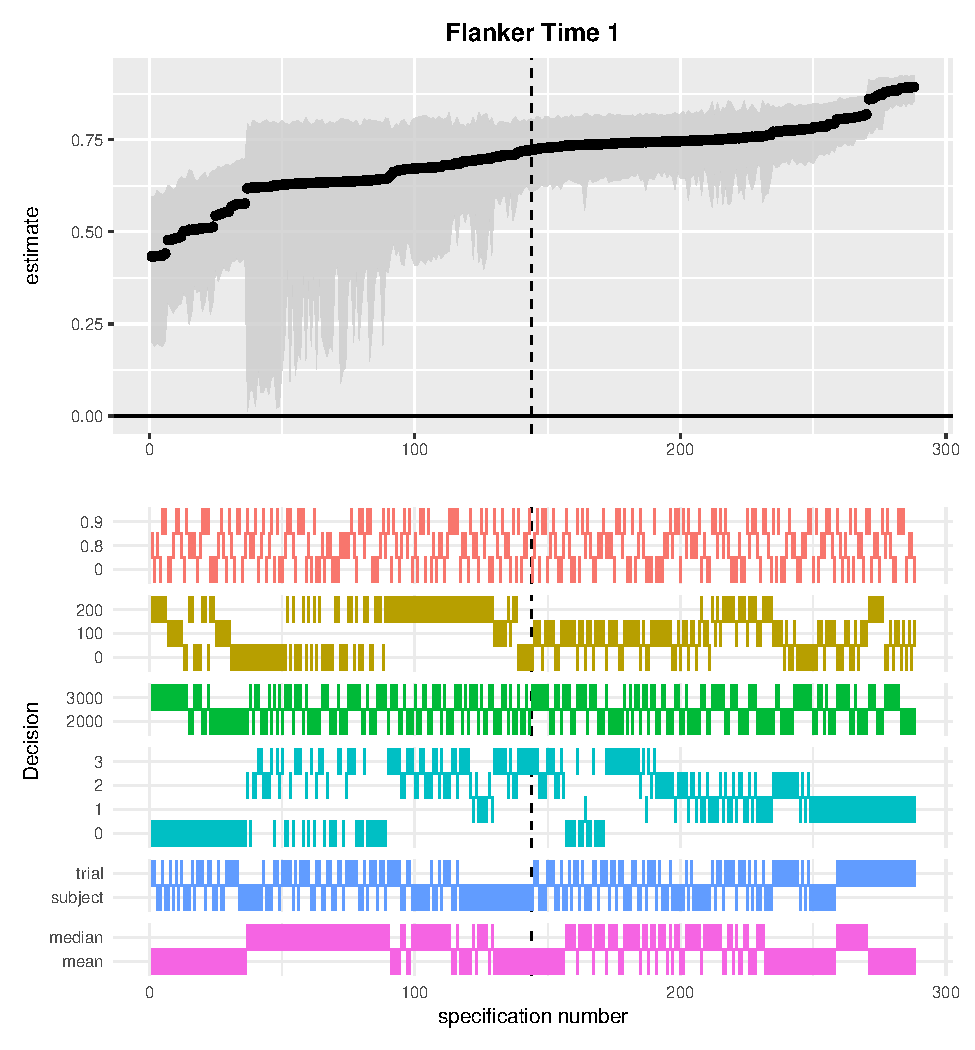
\includegraphics{half_trials_files/figure-latex/unnamed-chunk-4-1.pdf}
\caption{\label{fig:unnamed-chunk-4}Internal consistency reliability multiverse for Flanker RT cost at time 1}
\end{figure}

\begin{figure}
\centering
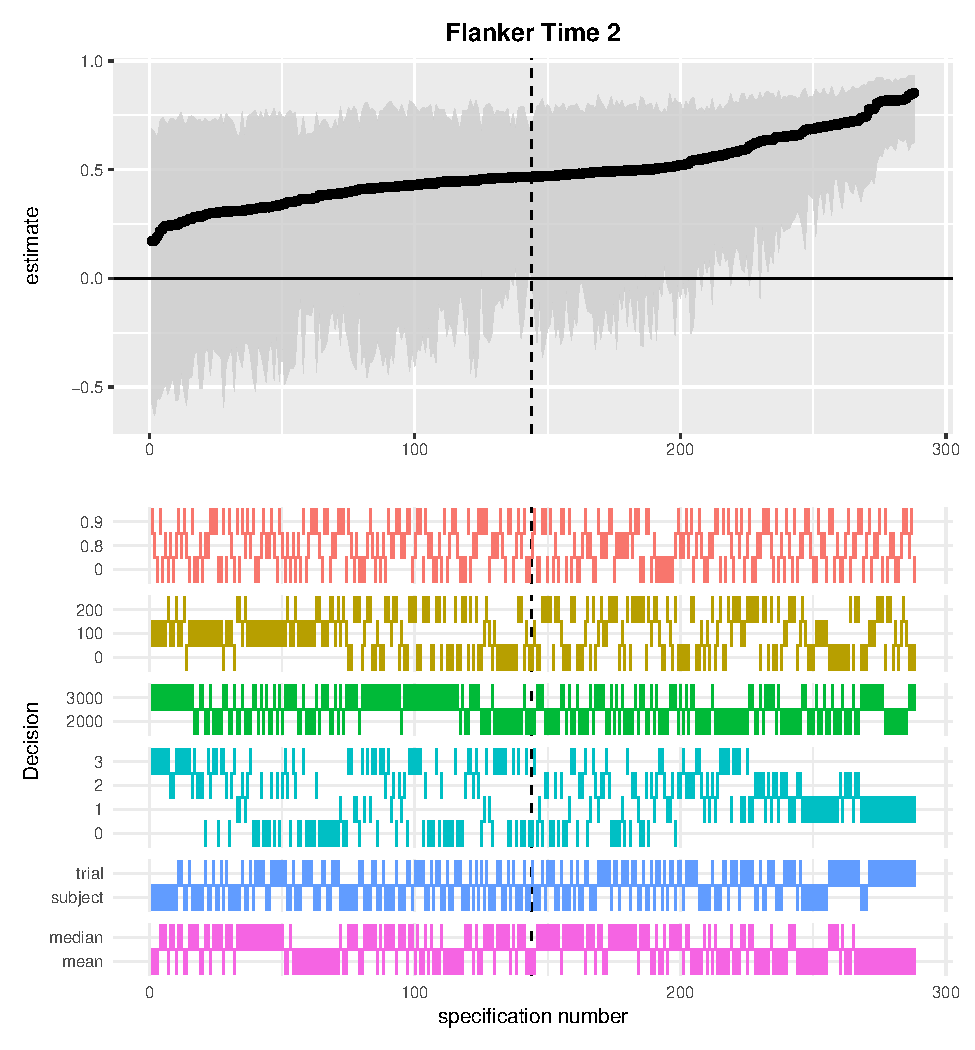
\includegraphics{half_trials_files/figure-latex/unnamed-chunk-5-1.pdf}
\caption{\label{fig:unnamed-chunk-5}Internal consistency reliability multiverse for Flanker RT cost at time 2}
\end{figure}

\begin{figure}
\centering
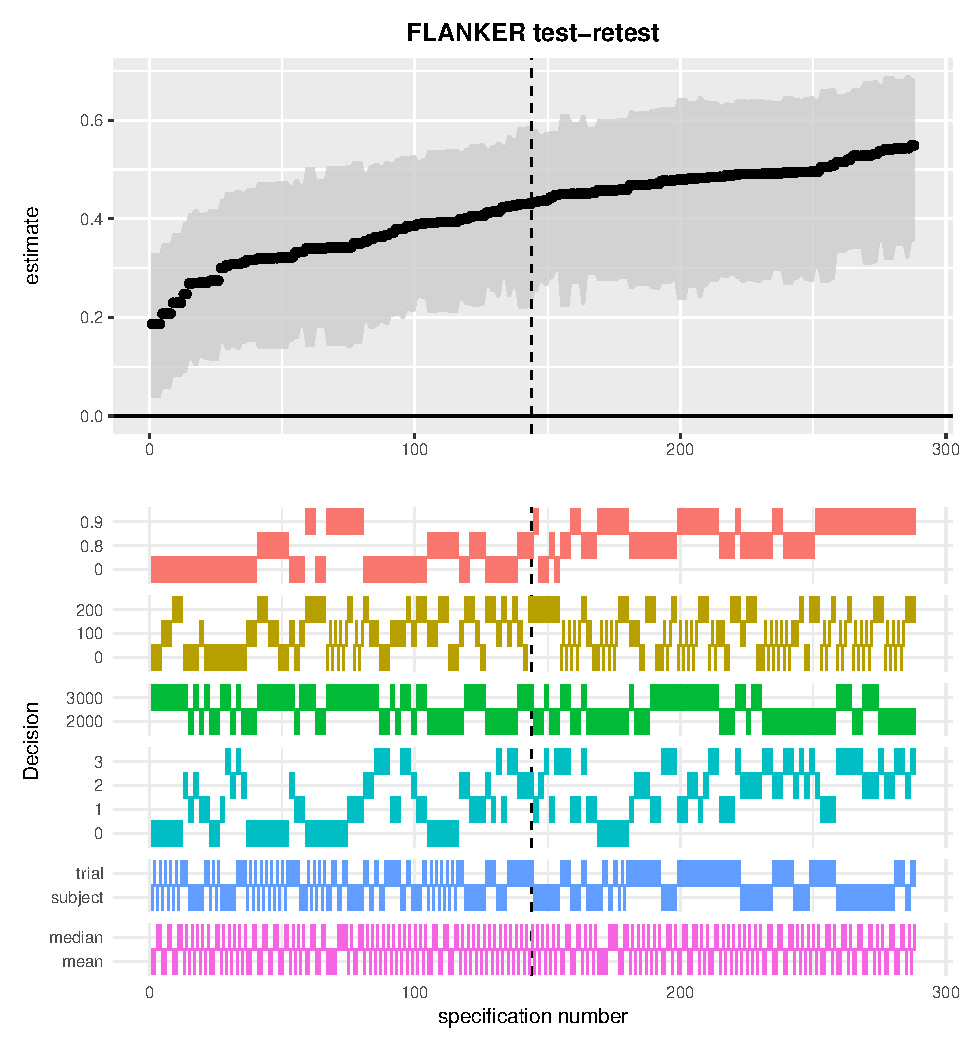
\includegraphics{half_trials_files/figure-latex/unnamed-chunk-6-1.pdf}
\caption{\label{fig:unnamed-chunk-6}Test-retest reliability multiverse for Flanker RT cost}
\end{figure}

\begin{figure}
\centering
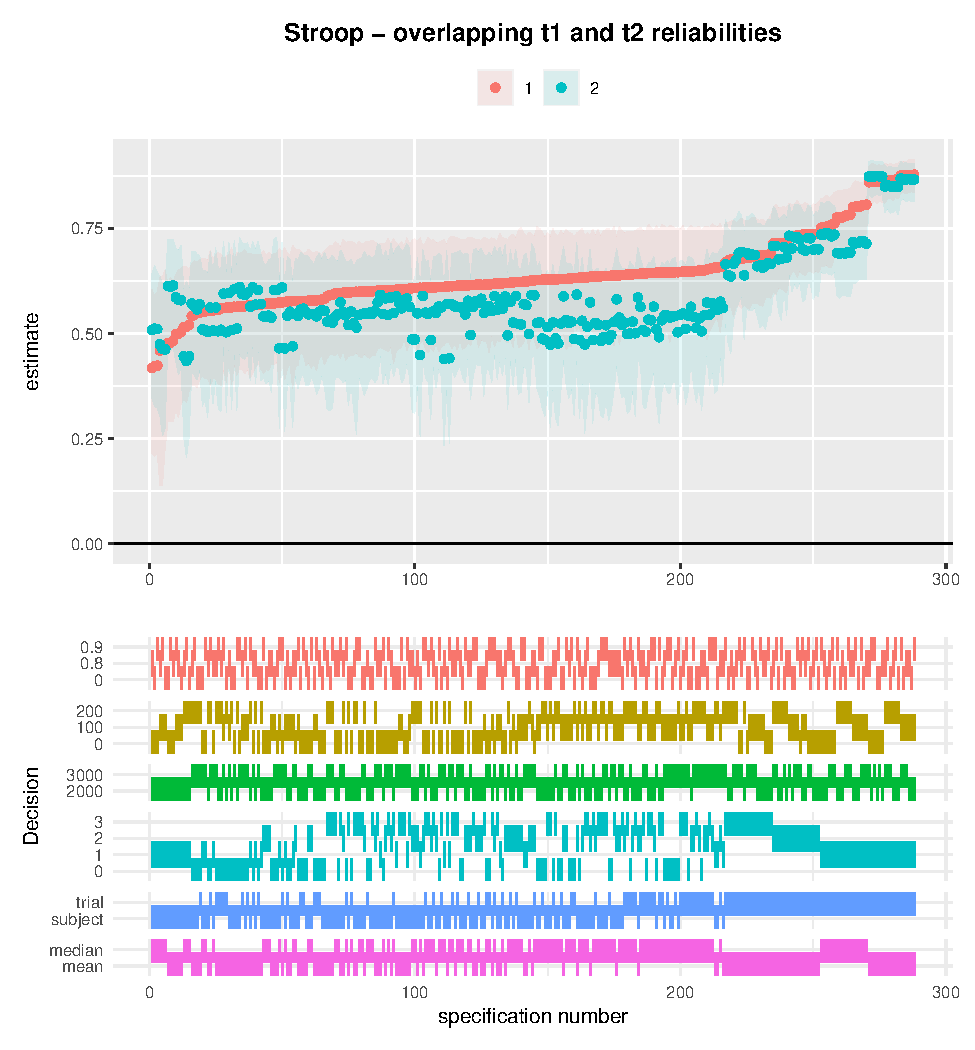
\includegraphics{half_trials_files/figure-latex/unnamed-chunk-7-1.pdf}
\caption{\label{fig:unnamed-chunk-7}Overlapped internal consistency reliability multiverse for Stroop RT cost at times 1 and 2}
\end{figure}

\begin{figure}
\centering
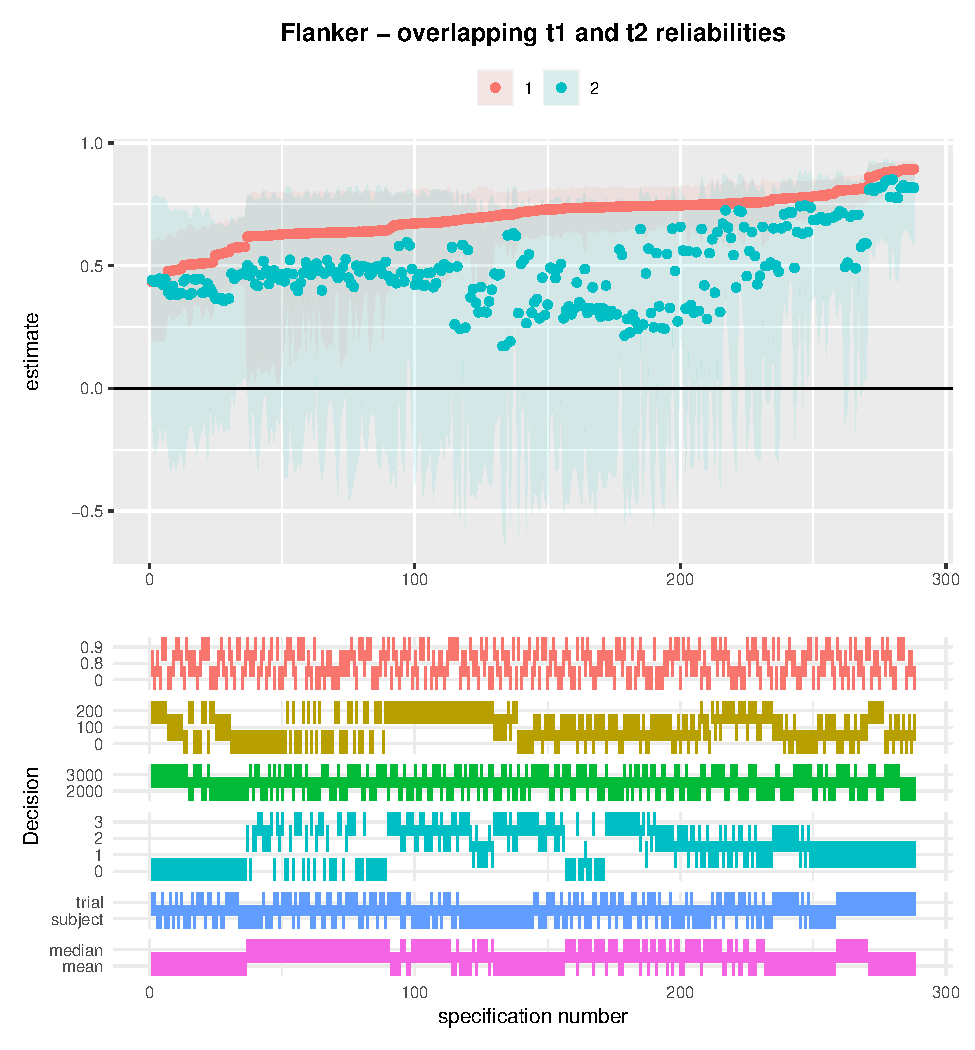
\includegraphics{half_trials_files/figure-latex/unnamed-chunk-8-1.pdf}
\caption{\label{fig:unnamed-chunk-8}Overlapped internal consistency reliability multiverse for Flanker RT cost at times 1 and 2}
\end{figure}

\begin{figure}
\centering
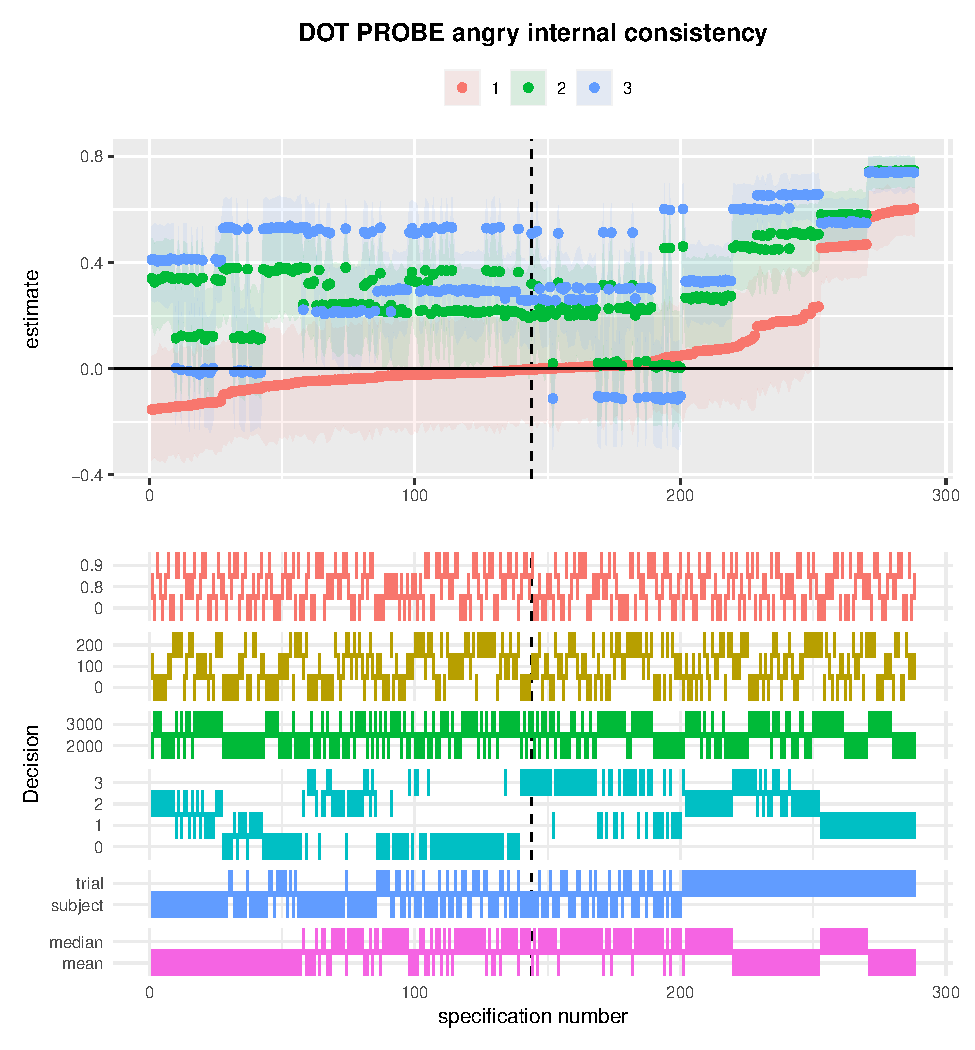
\includegraphics{half_trials_files/figure-latex/unnamed-chunk-9-1.pdf}
\caption{\label{fig:unnamed-chunk-9}Internal consistency reliability multiverse for Dot Probe attention bias (angry faces) at times 1, 2, and 3}
\end{figure}

\begin{figure}
\centering
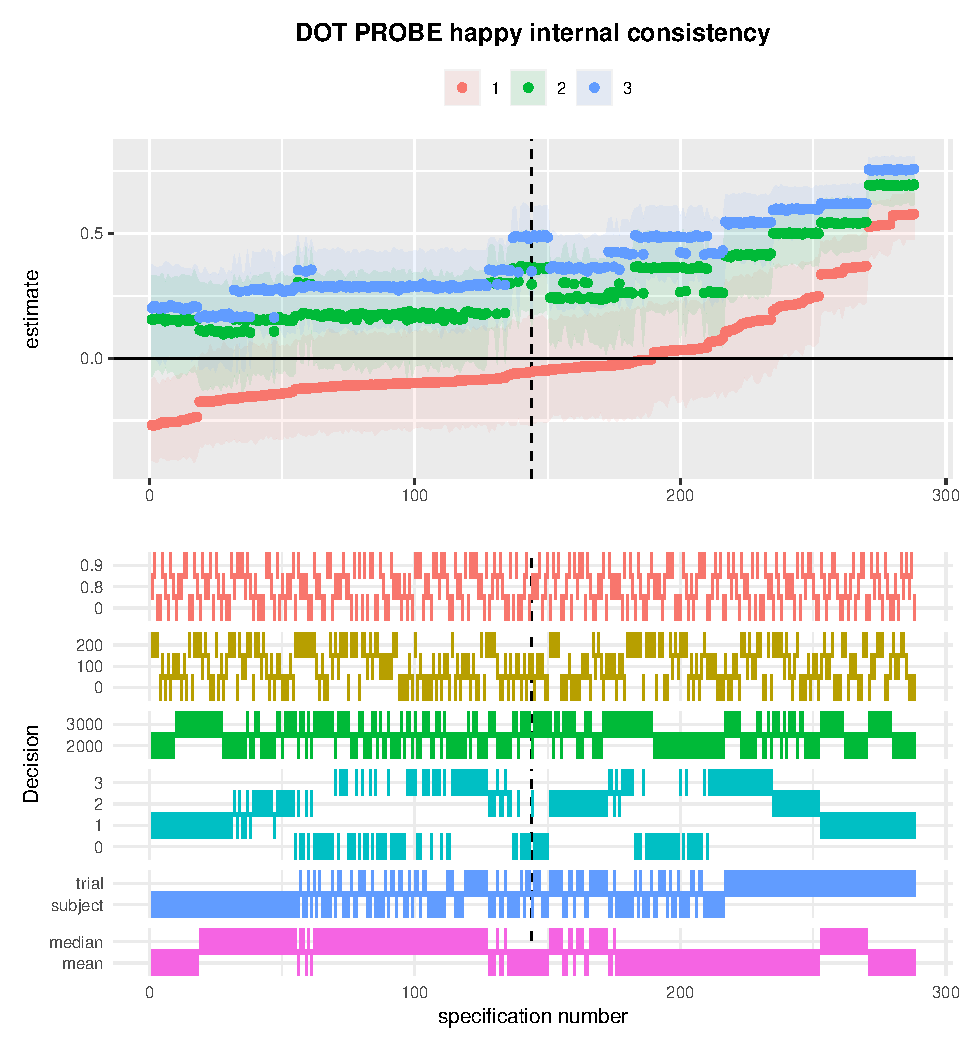
\includegraphics{half_trials_files/figure-latex/unnamed-chunk-10-1.pdf}
\caption{\label{fig:unnamed-chunk-10}Internal consistency reliability multiverse for Dot Probe attention bias (happy faces) at times 1, 2, and 3}
\end{figure}

\begin{figure}
\centering
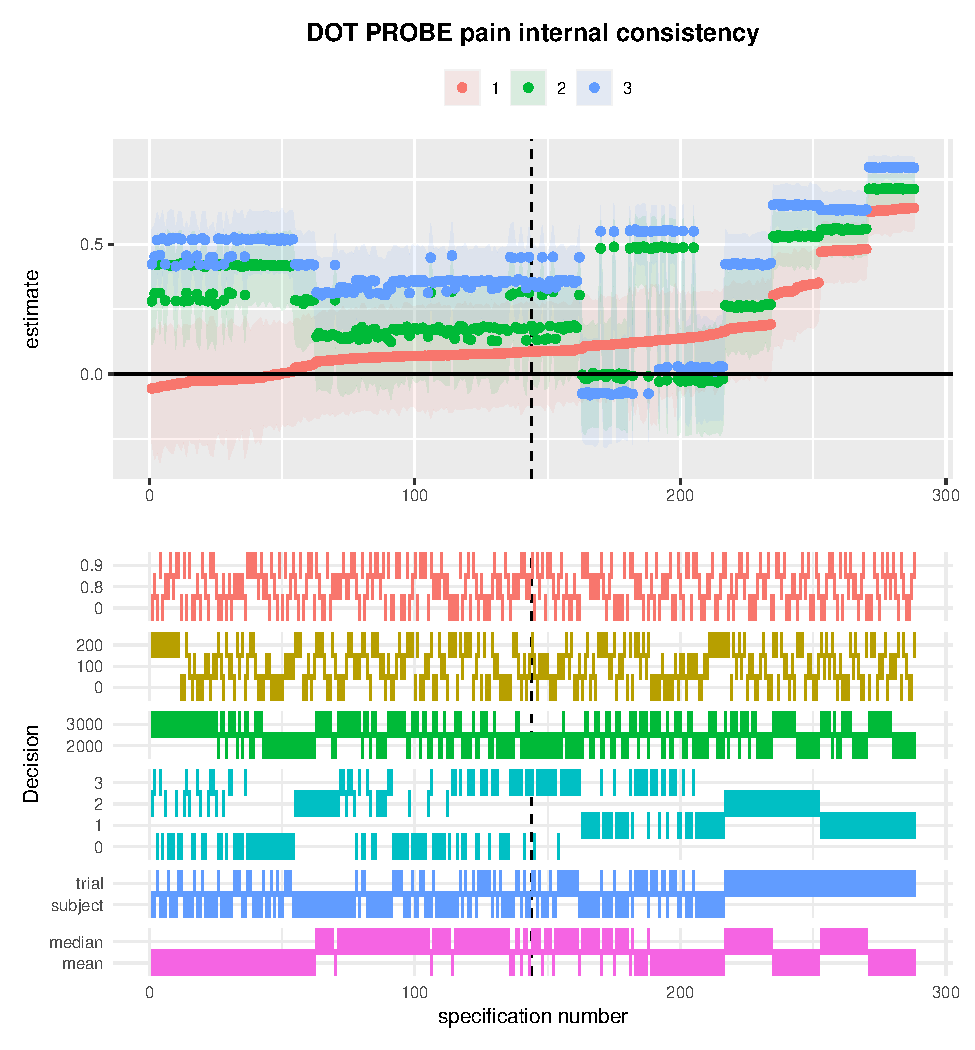
\includegraphics{half_trials_files/figure-latex/unnamed-chunk-11-1.pdf}
\caption{\label{fig:unnamed-chunk-11}Internal consistency reliability multiverse for Dot Probe attention bias (pain faces) at times 1, 2, and 3}
\end{figure}

\begin{figure}
\centering
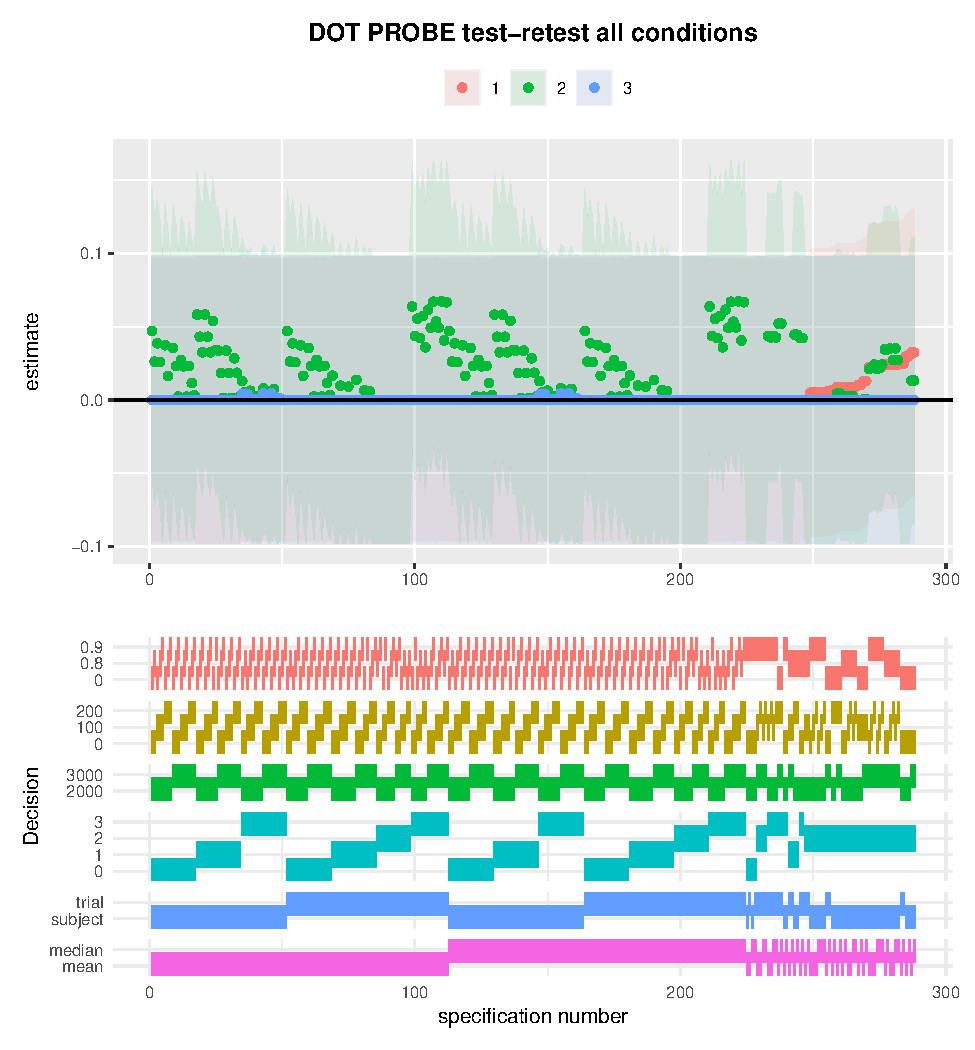
\includegraphics{half_trials_files/figure-latex/unnamed-chunk-13-1.pdf}
\caption{\label{fig:unnamed-chunk-13}Test-retest reliability multiverse for Dot Probe attention bias for all three conditions. Note: red = angry, green = happy, blue = pained}
\end{figure}

\begin{table}[tbp]

\begin{center}
\begin{threeparttable}

\caption{\label{tab:tableone}Correlations between reliability estimates and number of trials retained across specifications}

\begin{tabular}{lllrrr}
\toprule
task & \multicolumn{1}{c}{time} & \multicolumn{1}{c}{measure} & \multicolumn{1}{c}{correlation} & \multicolumn{1}{c}{95\% CI low} & \multicolumn{1}{c}{95\% CI high}\\
\midrule
Stroop & 1 & splithalf & -0.31 & -0.41 & -0.21\\
Stroop & 2 & splithalf & -0.42 & -0.51 & -0.32\\
Flanker & 1 & splithalf & -0.66 & -0.72 & -0.59\\
Flanker & 2 & splithalf & -0.59 & -0.66 & -0.51\\
DPTangry & 1 & splithalf & -0.57 & -0.64 & -0.49\\
DPTangry & 2 & splithalf & -0.17 & -0.28 & -0.05\\
DPTangry & 3 & splithalf & 0.20 & 0.08 & 0.30\\
DPThappy & 1 & splithalf & -0.36 & -0.46 & -0.25\\
DPThappy & 2 & splithalf & -0.31 & -0.41 & -0.20\\
DPThappy & 3 & splithalf & -0.15 & -0.27 & -0.04\\
DPTpain & 1 & splithalf & -0.68 & -0.74 & -0.61\\
DPTpain & 2 & splithalf & -0.07 & -0.18 & 0.05\\
DPTpain & 3 & splithalf & 0.17 & 0.05 & 0.28\\
Stroop &  & ICC & -0.38 & -0.47 & -0.27\\
Flanker &  & ICC & -0.52 & -0.60 & -0.43\\
DPTangry &  & ICC & 0.11 & 0.00 & 0.23\\
DPThappy &  & ICC & 0.13 & 0.01 & 0.24\\
DPTpain &  & ICC & 0.15 & 0.03 & 0.26\\
\bottomrule
\end{tabular}

\end{threeparttable}
\end{center}

\end{table}

\newpage

\begingroup
\setlength{\parindent}{-0.5in}
\setlength{\leftskip}{0.5in}

\hypertarget{refs}{}
\begin{CSLReferences}{0}{0}
\end{CSLReferences}

\endgroup


\end{document}
